\documentclass{article}
\usepackage[T1]{fontenc}
\usepackage{lmodern}
\usepackage{graphicx}
\usepackage{amsmath,amssymb}
\usepackage[a4paper,margin=2cm]{geometry}
\usepackage[absolute,overlay]{textpos}
\setlength{\TPHorizModule}{1mm}
\setlength{\TPVertModule}{1mm}
\usepackage[indonesian]{babel}
\usepackage{hyperref}
\setlength{\emergencystretch}{2em}
% unit: Halaman 15

\begin{document}

% === Halaman 15 (llm) ===

\section*{Pembentukan Kunci Putaran}

\begin{itemize}
    \item Kunci putaran ada sebanyak $2r + 2$ buah yang masing-masing disimpan di dalam elemen-elemen larik yang dilabeli sebagai $\text{S}[0], \text{S}[1], \dots, \text{S}[t - 1]$ dengan $t = 2r + 2$.
    \item Setiap elemen larik panjangnya satu \textit{word} ($1 \text{ word} = w \text{ bit}$)
\end{itemize}

\vspace{5mm}

% deskripsi: Tabel yang berisi parameter, simbol, dan nilai yang diperbolehkan untuk ukuran blok (w), jumlah putaran (r), dan panjang kunci eksternal K (b).
% bbox normalisasi: [0.1420, 0.6320, 0.7740, 0.8450]
\begin{textblock*}{132.72mm}(29.82mm,187.70mm)
\noindent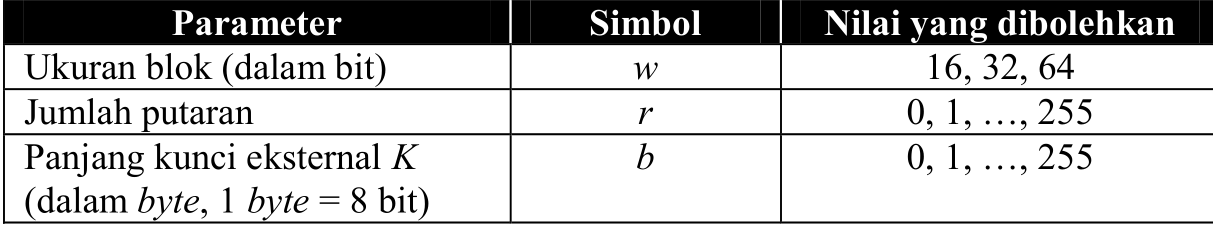
\includegraphics[width=132.72mm,height=63.26mm]{../../images/llm/page_015_img_01.png}%
\end{textblock*}

\end{document}
